\documentclass[11pt,a4paper]{article}

\usepackage[utf8]{inputenc}
\usepackage{amsmath}
\usepackage{amsfonts}
\usepackage{amssymb}
\usepackage{apacite} 
\usepackage{graphicx}
\usepackage{tikz}
\usepackage{fullpage}
\usepackage{listings}
\usepackage{perpage}
\usepackage{float}
\MakePerPage{footnote}
\usepackage[font=scriptsize,labelfont=bf]{caption}
\usepackage[left=2cm,right=2cm,top=2cm,bottom=2cm]{geometry}
\setlength{\parindent}{0pt} %indent set to 0 for now due to convenience and order

\usepackage[superscript,biblabel]{cite}
\makeatletter \renewcommand{\@citess}[1]{\textsuperscript{\,[#1]}} \makeatother %for brackets
\bibliographystyle{ieeetran}

\begin{document}

\title{Using Skynet to Calculate Charge State Abundances in Neutron Star Mergers}

\author{Pranav Nalamwar\\FRIB: \url{https://frib.msu.edu}\\Facility for Rare Isotope Beams\\Michigan State University\\Version: 0.04} 
\date{\today}
\maketitle

\begin{abstract}

The rapid-neutron capture process, or r-process, is behind the creation of the heaviest elements of the universe, such as the lanthanides. Neutron star mergers are the currently agreed upon site for the r-process to dominate in. Based on recent studies \cite{2017Natur.551...80K} , lanthanide abundances formed in the merger affect kilonovae light curves, where a kilonova is the culmination of the photons released by the merger material. Currently, there is an insufficient amount of energy level information available for the lanthanides, so we wanted to determine the significance of accurate atomic data on kilonova light curve calculations. To approach this, elemental abundances from Skynet, a nuclear reaction network code, was combined with NIST data on experimental and theoretical energy levels to calculate charge state abundance values via the Saha equation. The resulting charge state abundance values were successfully generated using NIST data, indicating any atomic data can be used for the calculations. These abundance patterns depict the transitions between dominating charge states, showing the importance of the energy levels. Thus, it is possible to compare the atomic models via comparing the resulting charge state abundance patterns and kilonovae light curves. 

\end{abstract}

\tableofcontents

\section{Motivation and Background}

\subsection{Stellar Nucleosynthesis}

Nucleosynthesis is the process by which the elements of the universe are created using only light nuclei formed after the Big Bang. \url{(https://journals.aps.org/rmp/abstract/10.1103/RevModPhys.29.547)} and \url{https://ui.adsabs.harvard.edu/abs/1955ApJ...121..144C/abstract}.  

The first stars (population III stars) were composed of primarily hydrogen and helium, and due to their massive sizes and pressures, were able to undergo nuclear fusion reactions and release heavier elements through supernovae. These elements include lithium, carbon, and other elements heavier than hydrogen and helium; when they are released by the supernovae, they enrich the chemical composition of the gas that will become part of a star in the future. This process continues to this day. \url{(https://www.physics.uu.se/ research/astronomy-and-space-physics/research/galaxies/\\first-stars-galaxies)}. 

Based on numerous observations of various stars, there are several types of stars, all of which undergo unique fusion reactions. For example, stars of roughly one solar mass stop fusing soon after the Carbon-Nitrogen-Oxygen (CNO) cycle is completed. As for heavier stars (20 to 50 solar masses), they will undergo numerous fusion reaction phases and layers before stopping at iron fusion. The last element formed in the core of the star is iron because the binding energy per nucleon of Fe-56 is the largest possible, meaning that fusion of these two nuclei is no longer energy efficient. Once that happens, a supernova event will proceed. Supernovae are thought to produce some elements heavier than iron through a neutron capture process. The lighter elements of the universe are formed through various channels, as seen by figure 1's elements categorized by origin.

\begin{figure}[h!]
  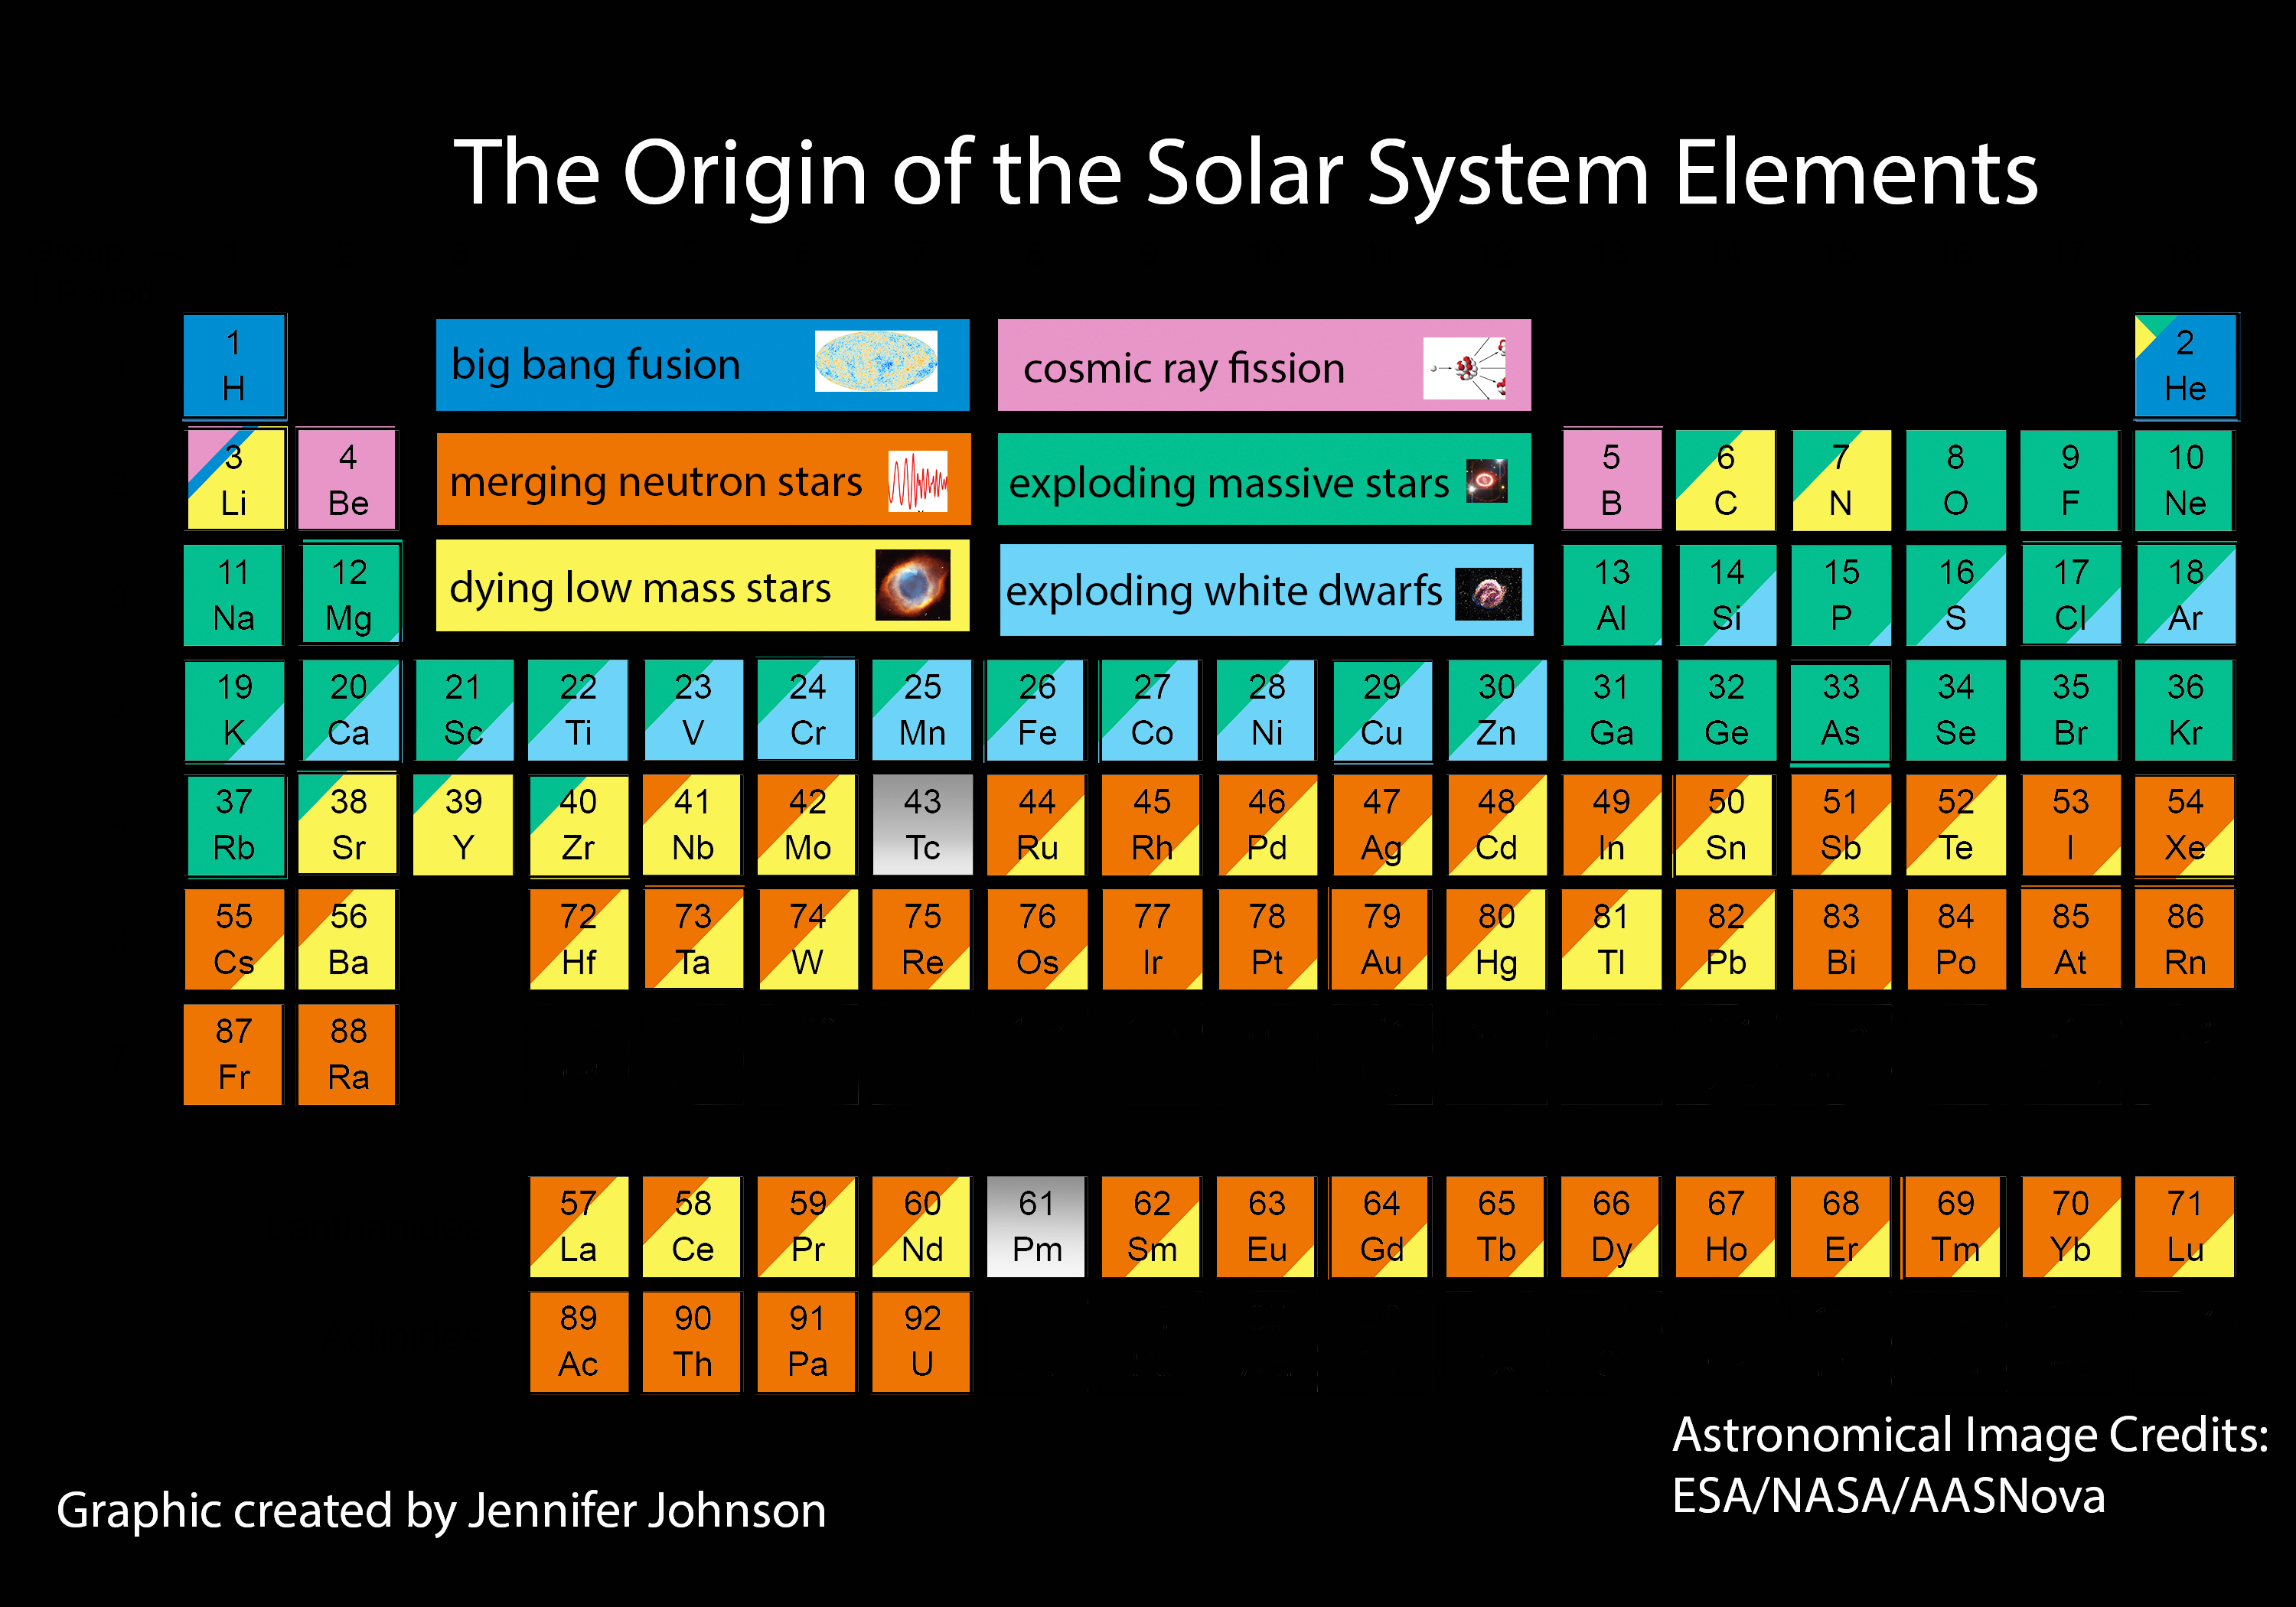
\includegraphics[width=1\textwidth]{periodic_table.png}
  \caption{Periodic table created by Jennifer Johnson depicting which elements are created by certain nucleosynthesis events, including neutron star mergers. \url{http://www.astronomy.ohio-state.edu/~jaj/nucleo/}}
\end{figure}

\subsection{The r-process}

Supernovae are considered a potential location for neutron capture as there is a fairly dense region of neutrons, which is necessary for the capture process. However, to create the heaviest elements in the universe, a highly dense region of neutrons are required, which facilitates the rapid neutron capture process, or r-process. It is considered rapid because the slow neutron capture process, or s-process, only involves nuclei absorbing one nuclei at a time before beta decaying. In comparison, the r-process involves seed nuclei such as iron-56 absorbing several neutrons in quick succession before eventually beta decaying back to stability, thereby resulting in nuclei that have higher charge and overall mass than the beginning. This progression is tracked by the various colors in the chart of the nuclides in figure 2. There are different nuclei made during this process, all of which can be found in the chart of the nuclides in figure 2, but simply put, this is how elements such as gold and uranium are theorized to have been produced in nature. While supernovae certainly contribute a fraction of the abundances of these elements found in nature, a better candidate for the r-process would be neutron star mergers. \url{(https://journals.aps.org/rmp/abstract/10.1103/RevModPhys.93.015002)}. The primary reasoning for this is because the neutrino flux present in supernovae, especially from the resulting stellar remnant, is high enough to reduce the number of neutrons present in the ejected material. As a result, the density of neutrons drop below what is needed to produce heavy r-process elements. In contrast, neutron star mergers can result in a wide variety of neutrino fluxes including low values.

\begin{figure}[h!]
  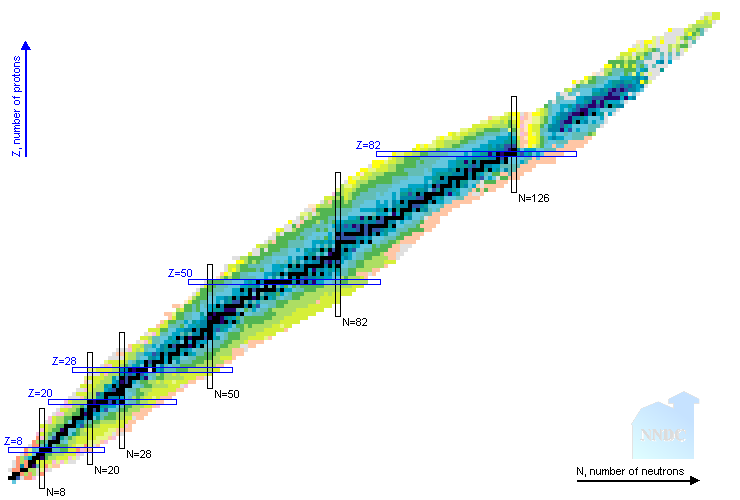
\includegraphics[width=1\textwidth , scale = .5]{nuclides_chart.png}
  \caption{Chart of the nuclides from the NNDC. It shows the set of all isotopes currently known, the decay process each isotope can undergo, the lifetime of each isotope. For the high N isotopes, the r-process becomes dominant, and the isotopes that are formed during the process is highlighted by the chart. These isotopes are the ones below the line of stability in black with more neutrons than protons. The various colors represent the stability of each isotope; the black blocks are stable isotopes and lighter colors represent isotopes that decay at quicker rates with light orange (high N and low Z), being the most unstable. The bars represent the stable magic numbers for isotopes based on the ratio of protons and neutrons present in the nucleus. \url{https://www.nndc.bnl.gov/nudat2/}}
\end{figure}

\subsection{Neutron Star Mergers}

Neutron star mergers (NSMs) are the coalescence of two dense balls of primarily neutrons typically only 10 km in diameter \url{(https://www.annualreviews.org/doi/abs/10.1146/annurev-nucl\\-013120-114541)}. As these neutron stars are mainly neutrons due to their immense densities and composition (95\% and 5\% protons), a merger between the two provides a dense source of neutrons ideal for the r-process. The residual nuclei, most of it being Fe-56, would have gone through several neutron absorptions and beta decays in short time spans before becoming fully stable. There is some observational evidence hinting that NSMs are indeed the site for the r-process, most notably GW170817 and its resulting kilonova AT 2017gfo as well as GRB 170817A. 


\subsection{Kilonovae Light Curves}

Kilonovae are one of two electromagnetic transients produced by neutron star mergers. The kilonova light curve, which shows the brightness over time of the event, often over all wavelengths, is composed of various spectra. The spectra's source includes a variety of elements, isotopes, and charge states, each of which can result in the emission of photons at different wavelengths. Example light curves indicating how the spectra is observed are shown in figures 3 and 4. The overall composition of the merger material dictates the properties of the light curve, namely its overall brightness, how long it peaks, and the time it peaks \url{(https://iopscience.iop.org/article/10.3847/2041-8213/ \\ aa9029/pdf)}.

The kilonova spectrum is composed of the spectra from the various elements in the mixture. These elements can be found in different charge states, such as neutral or +1 charge state. These charge states exist at certain temperatures, so several charge states can exist throughout the period the merger ejecta material cools. For a particular element existing in a particular charge state, there are many energy levels present that an electron can occupy, thereby resulting in transitions numbering in the thousands and above.\\

Unfortunately, due to this large forest of various spectra, it is difficult to ascertain what elements in which charge states were formed, so it is important to work backwards using models  \url{(https://iopscience.iop.org/article/10.3847/2041-8213/aa9029)}. The models can predict which groups of elements, whether it would be the transition metals or the lanthanides, are contributing certain spectral lines to the overall light curve. The lanthanides in particular are of course of great interest considering it is one of the least studied elements and the ones generated by r-process events \url{(https://iopscience.iop.org/article/10.1088/0004-637X/775/1/18)}.

\begin{figure}[h!]
  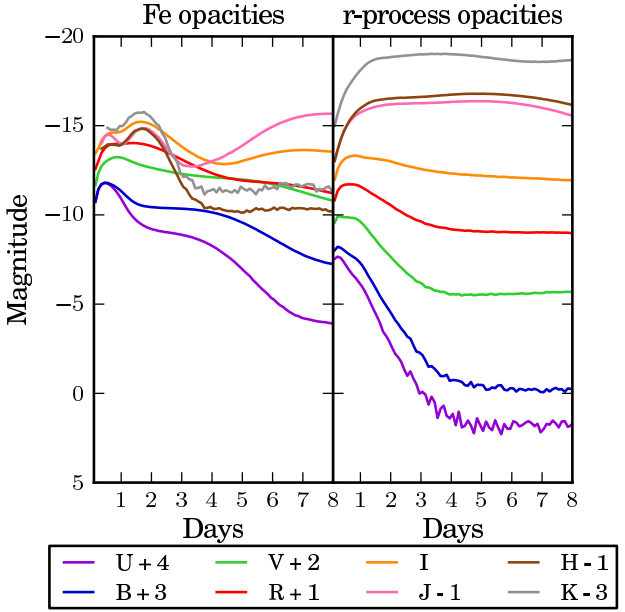
\includegraphics[width=1\textwidth]{light_curve.png}
  \caption{UV,optical, and near IR light curves for AT2017 gfo. The solid lines represent models that account for r-process heating and opacities while the shapes show observations. Thr three graphs on the right depict the same light curve over ten days for the g,i, and H light bands. \url{(https://iopscience.iop.org/article/10.3847/2041-8213/aa8fc7)} }
\end{figure}

The spectra from the lanthanides themselves are rather complex given that each of these elements has numerous valence electrons, and hence numerous energy levels and charge states present. However, through modeling, numerous studies have found that lanthanide abundances can have a measurable impact on the kilonova light curve \url{(https://academic.oup.com/mnras/article/441/4/3444/1223590 and \\ https://iopscience.iop.org/article/10.1088/0004-637X/775/1/18)}.

Specifically, it appears that a kilonova can be more "red" or "blue" depending on the lanthanide abundances. If the abundance is high, then the light curve is more red since the large density of lanthanides helps suppress most of the UV and optical light present from the merger mixture \url{(https://link.springer.com/ \\ article/10.1007\%2Fs41114-019-0024-0)}. In other words, the material has a high lanthanide opacity since the lanthanides makes the material opaque at the stated wavelengths. Opacity is defined as how efficient merger material is at absorbing radiation. On the other hand, a low abundance mixture will result in a bluer kilonova, which means that the light curve peaks, or is strongest, in the optical band. The opacity of the lanthanides is low, so the light from the UV/optical components is much easier to observe. Figure 5 indicates how changing the lanthanide fraction ultimately results in these bluer or redder light curves. 

\begin{figure}[h!]
  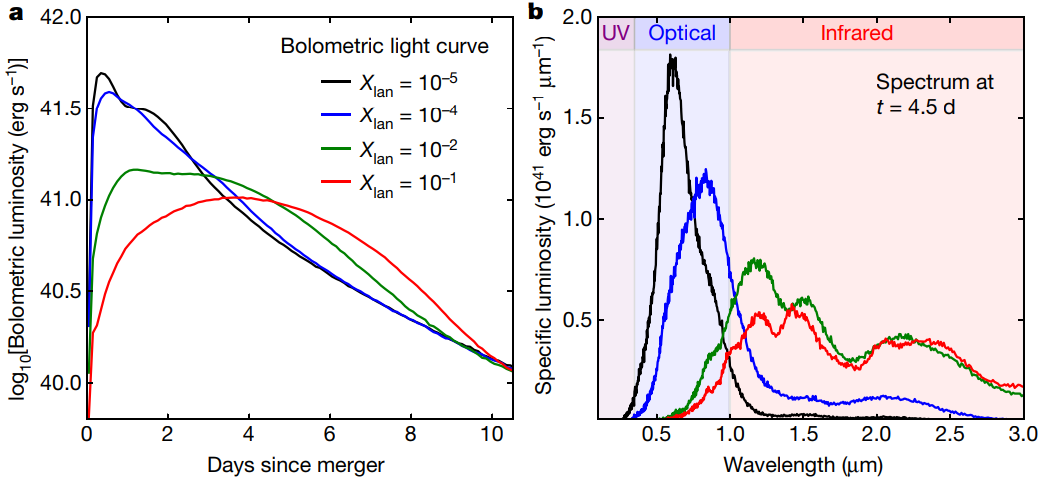
\includegraphics[width=1\textwidth]{kasen_curves.png}
  \caption{ Kilonova models for light curve(left). The graphic indicates the full bolometric luminosity vs days since merger for 10 days time. The various colors represent the lanthanide mass fraction present in the merger material, thus indicating that the lanthanide abundance can affect light curve on visible levels. The spectrum (right) shows the spectra observed from the merger at 4.5 days. Note that higher lanthanide fractions tend to shift the spectrum towards the IR. \url{(https://www-nature-com.proxy2.cl.msu.edu/articles/nature24453.pdf)} }
\end{figure}

While the information stated above had been known prior to the kilonova observation  AT2017gfo, several insights have been made as a result of studying this event. For one, AT2017gfo’s key features, especially its luminosity consistent to a blackbody, are all in agreement with predictions for kilonovae (\url{https://www.nature.com/articles/nature24453}).In a time less than 2 days after the merger, the emission is primarily dominated by the lighter r-process elements(bluer), but after 5 days, the emission is now dominated by the heavier r-process elements(redder). The infrared spectroscopy of the kilonovae provides even more compelling evidence for the creation of heavier elements, an idea indicated by the predictions for the spectral peaks of the merger matching observations. It was also found through observations that the decline of the luminosities in the g,r, and i bands of the light curve is unlike any other observations as they were much more rapid than that of supernovae \url{https://www.nature.com/articles/nature24291.pdf}. Specific observations include finding that the optical and infrared spectra agree with the fact that the early ejecta were mainly light r-process elements. There is a second spectrum suggesting Cs I and Te I could be possible light r-process elements that were created.Also, other potential candidates for forming in the merger would be neutral and singly ionized Xr and Sb I. The light curves and the spectra from this kilonovae indicate the ejecta is of high velocity, relatively low mass, and powered by a source that has similar timescales to the r-process \url{https://www.nature.com/articles/nature24303.pdf}. Pian et al.'s paper goes through the procedure for spectroscopic identification of many r-process elements in more detail \url{https://www.nature.com/articles/nature24298.pdf}.

\subsection{GW170817 Event and AT2017gfo Event}

GW170817 was a gravitational wave  detection by the Laser Interferometer for Gravitational Wave Observatory (LIGO) on August 17th, 2017. LIGO states the mass range of these stars was between 1.17 and 1.60 solar masses \url{(https://journals.aps.org/prl/abstract/10.1103/\\PhysRevLett.119.161101)}. It was established that this gravitational wave detection was indeed a neutron star merger event due to its component masses as well as the associated gamma ray burst. While this in itself was the first ever gravitational wave detection for a non-black hole based merger, it was also important due to its two associated optical components. 
First came a short Gamma Ray Burst (sGRB) approximately 1.7 seconds after the gravitational wave detection, also marking the first time gravitational waves and electromagnetic transients were both observed from the same astrophysical event. Figure 5 shows what telescopes saw in optical when observing GW170817's transients. It also points to the existence of light emitting atoms, which is also indicated by the kilonova AT 2017gfo. A kilonova, coined by Brian Metzger \url{(https://link.springer.com/article/10.1007\\/s41114-019-0024-0)}, is the emission of light by the excited atoms created by the r-process. These atoms interact with the electrons, cycling between bound and unbound states, resulting in photon emission. This ultimately results in a kilonova, which is indicative of what elements and charge states were created. 

\begin{figure}[h!]
  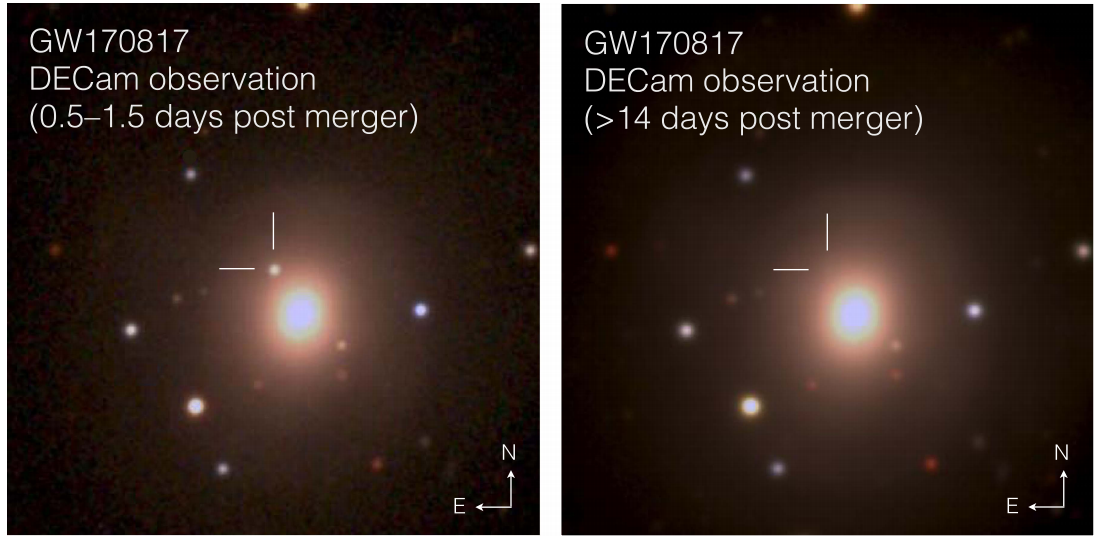
\includegraphics[scale = .5, width=1\textwidth]{GW170817_pic.png}
  \caption{Image of NGC4993, the galaxy containing the GW170817 event (left). It is a composite of the discovery image on August 17th 2017 at 00:05:23 and g and r color images taken at .5 and 1.5 days post merger. The other image (right) is the same but 14 days post merger. \url{(https://iopscience.iop.org/article/10.3847/2041-8213/aa9059)}}
\end{figure}


\subsection{Atomic Structure of Lanthanides}

The lanthanides are complex given their large nuclei and electrons. As a result, there is an array of isotopes and charge states available for each element. Since these lanthanides and their charge states are difficult to produce in a lab setting, scientists rely on atomic modeling, which requires accounting for the lanthanides' complexities. In the atomic modeling, it is necessary to calculate the various energy levels present to produce the light curve. However, each lanthanide has thousands of levels across the multiple charge states. Table 1 details these energy level complications. For example, Samarium has 63 charge states when including the neutral and fully ionized states; for just the first four states, there are 960 currently known energy levels according to the National Institute for Standards and Technology (NIST) database. The fifth state, which is the +4 charge state, only has two states known, which are the ground state and ionization energy. This means for Sm (V) and beyond, there is not much known experimentally or even theoretically. Therefore, modeling the lanthanides using atomic structure model calculations is necessary, albeit difficult. 

%Attempting to put in latex code for level table instead of screenshot or picture. Screenshot is better

\begin{table}[h!]
  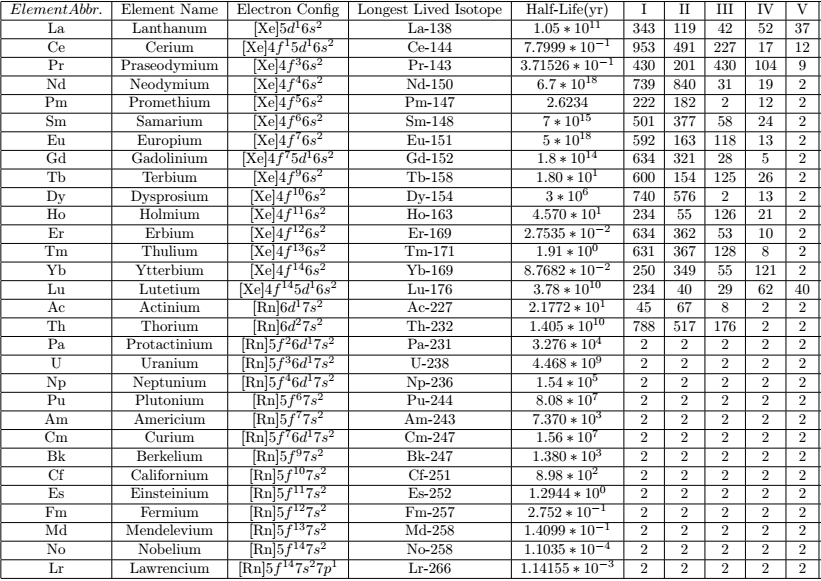
\includegraphics[width=1\textwidth]{level_pic.png}
  \caption{Table of lanthanides detailing number of atomic levels currently tabulated, which is necessary for spectra and opacity curves. Other key information such as electron configurations are listed. }
\end{table}

\pagebreak

\section{Calculating Charge State Abundances}

This chapter is dedicated to explaining how the charge state abundances used throughout the research is calculated, starting from Skynet’s elemental abundances. There are numerous tests and functions reliant on the charge state abundances. It will walk through the logic, reasoning, and pseudocode for each major coding section as well as graphics essential in illustrating key functions. 

It is important to calculate the charge state abundances since various charge states of the lanthanides exist in the ejecta material, all of which contribute the the spectra and thus the kilonova light curve. Thus, it is necessary to calculate how abundant each species is. Now to calculate these charge state abundances, the elemental abundances, a value calculated from Skynet via summing all the isotopic abundances of a given element together, is needed. Alongside the elemental abundance values, an accurate temperature vs. time extrapolation is needed to effectively calculate which charge state is present in the merger material at any give time. The temperature vs. time values are extrapolated since Skynet stops calculating the values once nuclear heating stops; since we deal with timescales of two weeks, well beyond Skynet's last temperature value, extrapolation is done. Together with this temperature and the elemental abundances, the charge state abundances are calculated via the Saha equation. 

\subsection{Introduction to Skynet}

Skynet, a nuclear-reaction network code for neutron star merger abundance calculations designed by Luke Roberts and Jonas Lippuner \url{(https://iopscience.iop.org/article/10.3847/\\1538-4365/aa94cb)}, is the starting point for the research. With certain initial parameters-- namely the electron fraction, dynamical time, and entropy-- we are able to calculate the abundances of various elements generated by neutron star mergers. Skynet is treated as a blackbox by only altering initial parameters. The electron fraction is the abundance of electrons present in the material either orbiting nuclei or freely moving in the ejecta material. The dynamical time is the timescale on which the ejecta will expand while the entropy is classically defined as the disorder of the system.

Note that abundances are measured in terms of the density or number of a given atom relative to the number or density of baryons present in the merger mixture. Skynet considers the nuclear data such as cross sections, the density of material and its temperature, and other factors to calculate this abundance information. Figure 6 is an example temperature-time plot produced by Skynet. It also outputs key data such as temperature, density, and electron fraction as functions of time, which are used for the charge state abundance calculations. The functions used for extracting data out of Skynet, primarily the abundance value ones since Skynet returns only isotopic abundances and we need elemental ones, is initialization(). Once the isotopic abundances are summed together to form the elemental abundances, a graph such as figure 7 is made to show the abundance vs time. 

\begin{figure}[h!]
  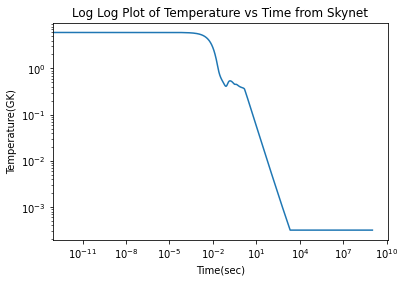
\includegraphics[scale = .75]{skynet_non_linear.png}
  \centering
  \caption{Plot of temperature vs time with temperature in units of GK. This is data extracted directly from Skynet. For large times, Skynet truncates any temperature calculation, resulting in this flat curve in late times. Temperature ranges from $10^1 \hspace{.03 cm} \mathrm{GK}$ to $10^{-4} \hspace{.03 cm} \mathrm{GK}$.}
\end{figure}

\begin{figure}[h!]
  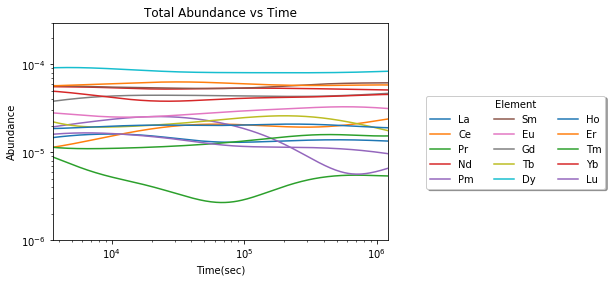
\includegraphics[scale = .65]{elemental.png}
  \centering
  \caption{Plot of abundances for all lanthanides over time (left) based on output from Skynet. Note that the abundances at early times is noise considering there are values lower than $10^{-20}$. Values become significant around $10^{-1}$ sec.}
\end{figure} 


\subsection{Extrapolating Temperature as a Function of Time from Skynet}

While Skynet does return the temperature and time of the merger material, it has a strong cutoff for very late times. This is because the goal for Skynet is to calculate what is produced by the end of the r-process instead of figuring out what elements and charge states are left once the material is fully cooled. Three temperature evolution models were created to address this cutoff issue and evolve the temperature past this point. The three models are based off what the material is assumed to be and how it evolves; the first is a radiation based adiabatic model, the second is a photon gas and is not adiabatic, and the last one involves both a photon gas and baryon component that are both non-adiabatic. The names of these models in the code are \\ temp \_ calculator(),  temp \_ evolution\_ photon(), and temp \_ evolution \_ baryon(). \\ 


\textbf{Radiation-Based, Adiabatic Model}: This is the simplest scenario where we take Skynet temperature data and apply a simple power law extrapolation. Here, we assumed that the system is purely radiation-dominated and adiabatic, which means there is no heat transfer present. Since Skynet has a cutoff temperature for late times, we first find the last unique temperature present. Using this and 300 temperature values before it, we fit the data to an equation of the form $y = mx + b$. In this scenario, the variables are all in log form. To find the slope $m$, we use two points along the line:

\begin{align}
	\dfrac{\Delta \log{T}}{\Delta \log{t}} = m 
\end{align}

where $T$ is the temperature in GK, and $t$ is the time in seconds. Using this slope and the current temperature value to calculate the next temperature. 

\begin{align}
	\log{T'} = m \left(\log{t' - t} \right) + log(T)
\end{align}

where $T$ is the current temperature, $t$ is the current time, and $T'$ is the next temperature value. Once this temperature is extrapolated, a temperature-time plot like figure 8 is created.  \\\\

\textbf{Photon Gas, Non-Adiabatic}: We now attempt to improve upon the first temperature evolution by assuming the composition consists of a photon gas, which implies that we can no longer use an adiabatic expansion here. Thus there is radiation and a photon gas. The radiation component refers to the photons that can do work on the system. The photon gas, on the other hand, refers to a collection of photons that acts like a gas, meaning it can be characterized by a pressure, temperature, volume, and entropy. We will derive a small change in temperature over a small change in time, which is later used in an ordinary differential equation solver to figure out the temperature evolution. This $\frac{dT}{dt}$ is based purely off data from Skynet. We first consider the entropy:

\begin{align}
	S = \dfrac{\lambda T^3}{\rho}
\end{align}

where $S$ is the entropy in $\mathrm{\dfrac{J}{kg \cdot sec \cdot GK}}$ , $T$ is the temperature in GK at a given timestep, $\rho$ is the density of the material in $\mathrm{\dfrac{kg}{m^3}}$, and the constant $\lambda$ as $\lambda =  \dfrac{4 \sigma_{sb}}{3}$, where the Stefan-Boltzmann constant $\sigma_{sb}$ has units of $\mathrm{\dfrac{J}{m^2 \cdot s \cdot {GK}^4}}$. We also know that 

\begin{align}
	\dfrac{dS}{dt} = \dfrac{\dot{Q} f}{T},
\end{align}

where $\dot{Q}$ is the heating rate in erg / s / g from Skynet, which is later converted to $\mathrm{\dfrac{J}{kg \cdot s}}$. The other value $f$ is an efficiency from 0 to 1 that represents how efficiently is the material heated. After taking the derivative of the defined value of $S$ from above, we set the two equations equal: 

$$ \dfrac{dS}{dt} = \dfrac{\dot{Q} f}{T} = \lambda \left(\dfrac{3T^2}{\rho}\dot{T} - \dfrac{T^3}{\rho^2}\dot{\rho} \right),$$ From here, we divide both sides by $f$ and distribute the $\lambda$
$$ \dfrac{3 \lambda T^2 \dot{T}}{f \rho} - \dfrac{T^3 \lambda}{f \rho^2}\dot{\rho} = \dfrac{\dot{Q}}{T}, $$

We then move the $\dot{\rho}$ term to the right 
$$ \dfrac{3 \lambda T^2 \dot{T}}{f \rho} = \dfrac{T^3 \lambda}{f \rho^2}\dot{\rho} + \dfrac{\dot{Q}}{T}, $$

We then divide by $\dfrac{3 \lambda T^2}{f \rho} $ to isolate $\dfrac{\dot{T}}{T}$
$$ \dfrac{\dot{T}}{T} = \dfrac{\dot{Q} f \rho}{3 \lambda T^4} + \dfrac{\dot{\rho}}{3 \rho} $$ 

Now note that since the density is homogeneous (uniform throughout), it can be written as $ \rho = \rho_0 \left(\dfrac{t}{t_0} \right)^{-3} $ where $\rho_0$ and $t_0$ are the initial densities and times, respectively. From this, we can get the derivative of $\rho$, which is $ \dot{\rho} = -3t^{-1} \rho $. 

With this, we can replace $\rho$ and $\dot{\rho}$ to get our equation.
$$ \dfrac{\dot{T}}{T} = \dfrac{\dot{Q} f \rho_0}{3 \lambda T^4} \left( \dfrac{t}{t_0} \right) ^{-3} - \dfrac{1}{t} $$ Finally, the temperature derivative can be written as 

\begin{align}
	\dot{T} = \dfrac{-T}{t} + \dfrac{\dot{Q} f \rho_0}{3 \lambda T^3} 	\left( \dfrac{t}{t_0} \right) ^{-3} 
\end{align}

This equation includes the original temperature-time evolution, which is the power law term, and the photon gas component, which is the second part of the equation. We can see there is a clear distinction between these terms.  This 
$\dot{T}$, an ODE, can be solved numerically to determine the temperature evolution, and the resulting graph is shown in figure 9.
\\\\

\textbf{Photon Gas and Baryon Component}: In this model, we now assume there is a radiation component, a photon gas component, as well as baryons and electrons that are part of this ejecta mixture. Due to the baryons, it is important to consider the pressures involved from radiation and the baryons themselves. Let us first use the first law of thermodynamics to define the derivative of the energy $\dfrac{d \epsilon}{dt}$ as

\begin{align}
	\dfrac{d \epsilon}{dt} = -P \dfrac{dv}{dt} + \dot{q}_\mathrm{nuc}
\end{align}

where $\epsilon, P, v, \dot{q}_\mathrm{nuc}$ are the energy of the system (this is energy per unit mass), the pressure, the specific volume (volume per unit mass), and the nuclear heating rate from r-process decays, respectively. Since $\rho$ is the mass density and $ v = \dfrac{1}{\rho} $ in the gas, then $ \dot{v} = \dfrac{dv}{dt} =  \dfrac{-1}{\rho ^2}\dot{\rho} $. With these substitutions, $\dot{\epsilon}$ becomes: 

\begin{align}
	\dfrac{d \epsilon}{dt} = \dfrac{4a T^3}{\rho} \dot{T} - 			\dfrac{a T^4}{\rho^2}\dot{\rho} 
\end{align}

We can also write the energy in another way; both the photon gas and baryon/electrons components have energy values. The photon gas energy is given by $\epsilon_{\gamma} =\dfrac{a T^4}{\rho}$, where $a$ is the radiation constant defined as $a = \dfrac{4 \sigma_{sb}}{c}$ with units of $\mathrm{\dfrac{J}{m^3 \cdot {GK}^4}}$.\\

The baryon and electron energy, which we will denote as the non-radiation energy, is given by $\epsilon_{non-rad} = \dfrac{3 k_B T}{2 m_p} Y_{non-rad}$. Now $k_B, m_p$ are the Boltzmann constant and the baryon mass, respectively. $Y_{non-rad}$ is just a placeholder abundance value to show the density of particles present. The sum of these energies, $\epsilon_{tot} = \epsilon_\gamma + \epsilon_{non-rad}$ will give us the total energy. 
\\

From here, we can rewrite $Y_{non-rad}$ with the abundance values from the atoms and electrons as well as rewrite $\epsilon_{tot}$. This equation becomes:  

\begin{align}
	\epsilon_{tot} = \dfrac{a T^4}{\rho} + \dfrac{3 k_B T}{2 m_p} \left[\sum_{i=0}^{Z} Y_i(t) + Y_e \right] 
\end{align}

This equation's first term is the radiation energy component while the second term is for the baryons and electrons. These baryons and electrons make up the non-radiation component mentioned earlier. The non-radiation component consists of the baryons, which are found in nuclei and affect the elemental abundance values $Y_i$. The electrons are either orbiting the nucleus or are free-floating, so the electron fraction term $Y_e$ is used here as the sum of all electrons present in the ejecta. The baryon mass is chosen to be the proton mass for convenience. The term in the bracket inside equation 8 will be denoted as $\tilde{Y}$ for convenience.\\
We now take the derivative of this energy equation, leading to the following expression. \\

$$ \dfrac{d \epsilon}{dt} = \dfrac{4a T^3}{\rho}\dot{T} - \dfrac{a T^4}{\rho^2} \dot{\rho} + \dfrac{3 k_B}{2 m_p} \tilde{Y} \dot{T} + \dfrac{3 k_B}{2 m_p} T \tilde{\dot{Y}} $$ \\

We now solve for $\dfrac{dT}{dt}$ to find: 
$$ \dfrac{P}{\rho^2} \dot{\rho} + \dot{q_{nuc}} = \dfrac{4a T^3}{\rho} \dot{T} -  \dfrac{aT^4}{\rho^2} \dot{\rho} + \dfrac{3 k_B}{2 m_p} \dot{T} \tilde{Y} + \dfrac{3 k_B}{2 m_p} T \dot{\tilde{Y}} $$ From here, we can solve for $\dfrac{dT}{dt}$, which is 

\begin{align}
	\dfrac{dT}{dt} = \dfrac{[ \dfrac{P}{\rho^2} \dot{\rho} + \dot{q_{nuc}} + \dfrac{aT^4}{\rho^2} \dot{\rho} - \dfrac{3 k_B}{2 m_p} T \dot{\tilde{Y}}]} {[\dfrac{4a T^3}{\rho} + \dfrac{3 k_b}{2 m_p} \tilde{Y}]}
\end{align}

This equation presents the temperature derivative in terms of known values except for the pressure. We now need to determine the pressure $P$ in terms of Skynet's output parameters. Thus, we know that the total pressure, $P_{tot}$, is given as $P_{tot} = P_{\gamma} + P_{ideal}$. Since the specific volume is $v = \dfrac{1}{\rho}$ and the pressure is related to the energy by $P_\gamma = \frac{U}{3V}$,  we get the radiation pressure $P_{\gamma} = \dfrac{a T^4}{3}$.\\
Now the ideal gas pressure is a result of all the baryons in the ejecta, which is usually defined as $P_\mathrm{ideal} = \dfrac{N k_b T}{v}$, where $N$ is the total number of baryons present. The total number of particles comes from the abundance of species $Y_i = \dfrac{n_i}{n_B}$, where $n_i = \dfrac{N_i}{v}$. Note that $n_B$ is the number density of baryons present. Thus, we can now calculate the ideal gas pressure: For a given species i,
$$ P_i = Y_i n_B k_b T  = Y_i \rho k_b T$$ Now since $\rho = m_p n_B$, we then can write $P_i = \dfrac{Y_i \rho k_b T}{m_p}$. Putting all the ideal gas components together, we can write 
$$ P_{ideal} = \sum_{i=0}^{Z} P_i + \dfrac{Y_e \rho k_b T}{m_p} $$ The total pressure, written with $\tilde{Y}$, is:

\begin{align}
	P_\mathrm{tot} = \dfrac{a T^4}{3} + \dfrac{\tilde{Y} \rho k_b T}{m_p}
\end{align} 

Finally, we can write $\dot{T}$ in terms of known values as 

\begin{align}
	\dfrac{dT}{dt} = \dot{T} = \dfrac{ \left(\dfrac{4 a T^4}{3} + \dfrac{\tilde{Y} \rho k_b T}{m_p} \right) \dfrac{\dot{\rho}}{\rho ^2} + \dot{q}_{nuc} - \dfrac{3 k_b}{2 m_p} T \dot{\tilde{Y}}} { \left( \dfrac{4a T^3}{\rho}  + \dfrac{3 k_b}{2 m_p} \tilde{Y} \right)}
\end{align}

With this equation, we know that the temperature evolution is dependent on $Y_i, Y_e, \rho, T, \dot{q_{nuc}, \dot{\rho}}$. Note that $\dot{\tilde{Y}}$ is not calculated or calculated only through a simple derivative of the form $\dot{\tilde{Y}} = \dfrac{d \tilde{Y}} {dt} $. This is because, for late times, the nuclear heating has cooled to the point where elemental abundances are approximately constant. Thus, for convenience, the calculations often set $\dot{\tilde{Y}} = 0$. \\

We can further simplify our above expression by removing the density. Since our ejecta material is assumed to be homogenous,  $\rho = \rho_0 \left(\dfrac{t}{t_0}\right)^{-3}$ and $\dot{\rho} = \dfrac{-3 \rho}{t}$, we can rewrite equation (11) as:

\begin{align}
	\dfrac{dT}{dt} =  \dfrac{ -\left( \dfrac{4aT^4}{3 \rho_0} \left (\dfrac{t}{t_0} \right)^3 + \dfrac{k_b T \tilde{Y}}{m_p} \right) \dfrac{3}{t} - \dfrac{3 k_b T \tilde{Y}}{2 m_p} \dfrac{\dot{\tilde{Y}}}{\tilde{Y}} + \dot{q}_{nuc} } {  \left( \dfrac{4 a T^3}{\rho_0} \dfrac{t}{t_0}^3 + \dfrac{3 k_b \tilde{Y}}{2 m_p}\right) }
\end{align}

The above equation is the solution since it was assumed that the density, and therefore its derivative, were homogenous and homologous. Homologous means the material, to first order at least, has the same properties such as temperature and density throughout.  Thus, we now have $\dot{T}$ is a function of $(T,t,\tilde{Y}, \dot{\tilde{Y}},\dot{q}_{nuc})$, which are all outputs of Skynet, except for $\dot{\tilde{Y}}$, which is calculated from taking the derivative of the abundances outputted. $T$ is in units of $\mathrm{GK}$, $t$ is in $\mathrm{sec}$, $\tilde{Y}$ is unitless, $\dot{\tilde{Y}}$ is in units of $\dfrac{1}{\mathrm{sec}}$, $\dot{q}_{\mathrm{nuc}}$ is initially in $\dfrac{\mathrm{erg}}{\mathrm{sec \cdot g}}$ but later converted to $\dfrac{J}{\mathrm{kg \cdot sec}}$, and $\rho_0$ is initially in $\dfrac{\mathrm{g}}{{\mathrm{cm}}^3}$ but is later turned into $\dfrac{\mathrm{kg}}{\mathrm{m}^3}$. The resulting temperature-time plot from solving the ODE outlined in equation 12 is shown in figure 10. Relative to figures 8 and 9, there is a deviation of less than one order of magnitude. Nonetheless, this deviation does warrant calculating the charge state abundance values using this new temperature-time relationship. \\


\begin{figure}[h!]
  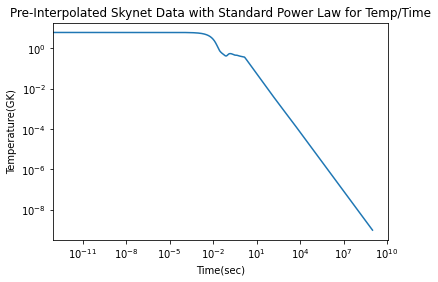
\includegraphics[scale = .7]{linear_temp.png}
  \centering
  \caption{Plot of temperature vs time after applying the radiation-based, adiabatic model. Notice how it becomes fully linear in log-log space.}
\end{figure} 

\begin{figure}[h!]
  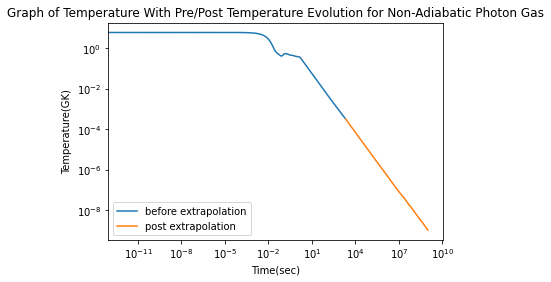
\includegraphics[scale = .7]{photon_only.png}
  \centering
  \caption{Plot of temperature vs time after applying the photon-gas, non-adiabatic model. Notice how there is no interruption in the linearity of the temperature/time plot in log-log space.}
\end{figure} 

\begin{figure}[H]
  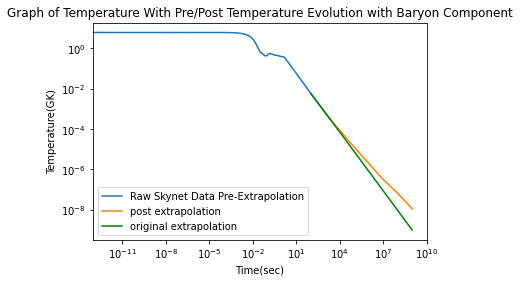
\includegraphics[scale = .7]{photon_baryon.png}
  \centering
  \caption{Plot of temperature vs time for an ejecta with a radiation, photon gas, and baryon component. For the same dataset as the other temperature evolution models, this new extrapolation varies slightly relative to the radiation-only model. In other words, the orange line varies less than an order of magnitude in temperature relative to the original extrapolation. }
\end{figure} 

\pagebreak

\subsection{Solving the Saha Equation}

The Saha equation, named after Meghnad Saha, is used to calculate the relative abundance between two charge states of a given element based on the current temperature and electron fraction present in the merger material \url{(https://archive.org/details/plasmachemistry00frid)}. Now we know that all the charge state abundances together form the full elemental abundance of a given element output by Skynet. This is crucial since all the relative abundances calculated by the Saha equation can be summed together and checked with the total elemental abundances from Skynet. Note that the Saha equation utilizes the ionization energy for each charge state, a value that is either found theoretically or experimentally for the lanthanides due to their rarity and short half-lives. It is also difficult to find the electron fraction, which is the density of electrons in the mixture relative to the total number of baryons present. The electron fraction $Y_e$ in the Saha equation is actually the free electron fraction $Y_{e,free}$, or the density of electrons that are freely moving instead of being in orbit about some nucleus in an atom. The saha and saha \_ mult classes go into depth about how to implement the Saha equation with these constraints in mind.  \\



We start with the constraint on the element abundances of element $Z$, where the element is determined purely by the number of protons. Essentially, for a given time step, the sum of all charge state abundances must equal the elemental abundance provided by Skynet. Technically, Skynet provides data in isotopic abundances, so the sum of the isotopic abundances of any element is the elemental abundance. The same principle applies to the charge states; the sum of the charge state abundances $Y_{Z,I}$ make up the elemental abundance $Y_Z$.

$$Y_Z (t) = \sum_{I=0}^{Z} Y_{Z,I}(t)$$

$Y_Z (t)$ is the total abundance of element $Z$ and $Y_{Z,I}$ is the abundance of $Z$ in charge state $I$. To calculate the bound electron fraction from here, we need to know the abundance of all the charge states of all elements involved since nuclei have electrons orbiting them. 
\\\\
$$Y_{e,bound} = \sum_{Z=0}^{Z_{max}} \sum_{I=0}^{Z} (Z - I) Y_{Z,I}(t) = (1-f) Y_{e,tot}(t) $$

$Z_{max}$ is for summing over all possible elements while the second sum is summing over all possible charge states of $Z$. 
\\The value of $f$ is introduced such that $Y_{e,free} = f \hspace{.1mm} Y_{e,tot}$, where $Y_{e,free}$ is the free electron fraction and $Y_{e,tot}$ is the total electron fraction in the mixture, both of which are fractions between 0 and 1. \\

Let's now look at the Saha equation, which is converted to abundances rather than densities: 

\begin{align}
\frac{Y_{Z,I+1}}{Y_{Z,I}}  = \frac{2}{\rho N_A  Y_{e,tot} f}  \left(\frac{G_{Z,I+1}}{G_{Z,I}}\right) \left(\frac{m_e k_b T}{2\pi\hbar^2}\right)^\frac{3}{2} \scalebox{1.3} e^{\left(\dfrac{\displaystyle -\chi_i}{\displaystyle k_b T}\right)}  
\end{align}

Here, $\rho $ is the density of outgoing ejecta in $\mathrm{\dfrac{g}{cm^3}}$, $N_A = $ Avogadro's Number = $6.02214076 \hspace{1mm} \mathrm{x} \hspace{1mm} 10^{23} \hspace{.1 cm} $ $\mathrm{mol^{-1}}$,  $m_e = $ mass of an electron, $9.109 \hspace{1mm} \mathrm{x} \hspace{1mm} 10^{-28} \hspace{.1 cm} \mathrm{g} $, $k_b = $ Boltzman Constant = $1.38064852 \hspace{1mm} \mathrm{x} \hspace{1mm} 10^{-16} \hspace{.1 cm} \mathrm{\dfrac{erg}{K}}$, $T = $ temperature in $\mathrm{GK}$, $\hbar = $ Reduced Planck's Constant = $1.0545 \hspace{1mm} \mathrm{x} \hspace{1mm} 10^{-27} \hspace{.1cm} \mathrm{erg \cdot s}$, and $\chi_i = $ Ionization Potential in $\mathrm{eV}$.\\
 
The function $G$ is the partition function, a number that indicates how many microstates or arrangements are possible. However, since most of these states are unknown, we assume the partition function ratio is of order 1. We will condense the entire right side of the equation into a function $g_i (\rho,Y_{e,tot},T) $ such that we get 

\begin{align} 
g_i \equiv \dfrac{2}{\rho N_A  Y_{e,tot} f}  \left(\dfrac{G_{Z,I+1}}{G_{Z,I}}\right) \left(\dfrac{m_e k_b T}{2\pi\hbar^2}\right)^\frac{3}{2} \scalebox{1.3} e^{\left(\dfrac{\displaystyle -\chi_i}{\displaystyle k_b T}\right)}.
\end{align}

We will now rewrite the Saha equation in a form easier to use for calculating the abundances values

$$ Y_{Z,I+1} = Y_{Z,I} \cdot g_I \Longrightarrow  Y_{Z,1} = Y_{Z,0} \cdot g_0 $$   $$ Y_{Z,2} = Y_{Z,1} \cdot g_1 = Y_{Z,0} \cdot g_1 \cdot g_0 $$

We can then generalize this to any state: 

\begin{align} 
Y_{Z,I} = Y_{Z,0} \prod_{m=0}^{I - 1} g_m 
\end{align}

Also, we put a constraint on $Y_Z$, namely that all the charge state abundances make up the elemental abundance.  

$$ Y_Z = \sum_{I=0}^{Z} Y_{Z,0} \left(\prod_{m=0}^{I - 1} g_m\right) $$\\
\begin{align} 
\Longrightarrow Y_{Z,0} = \frac{Y_Z}{\quad \displaystyle \sum_{I=0}^{Z} \medspace \prod_{m=0}^{I - 1} g_m}
\end{align}

Note that the right hand side of the equation can be calculated purely from Skynet output and data about ionization potentials, which means you can use the above two equations to get all the $Y_{Z,I}$ for a single $Z$. 
\\
In total, you have an abundance calculation function that is dependent on the following parameters:

$$\mathrm{func}(T,\thinspace p,\thinspace Y_{e,free},\thinspace [\chi_i],\thinspace Y_Z)$$

While these equations are correct, high temperatures result in large $g_m$ values, resulting in either overflow or underflow issues. In other words, there is a normalization issue. Therefore, instead of altering the charge state each time $g_m$ is calculated, we focus on just one charge state at a time and normalize with this one state only. 

First we rewrite the expression  $\thinspace \displaystyle \prod_{m=0}^{I - 1} g_m$ as $h_I$, which is a function of $T,\thinspace p,\thinspace Y_{e,free}$. \\

As a result, we see that $Y_{Z,I} = h_I  Y_{Z,0}$. Now say another charge state $j$ is chosen, thus $Y_{Z,J} = h_J  Y_{Z,0}$. \\

Therefore, the following relation is true:
$\frac{Y_{Z,I}}{Y_{Z,J}} = \frac{h_I}{h_J} $ $\Longrightarrow
Y_{Z,I} = Y_{Z,J}\thinspace \frac{h_I}{h_J}$. \\

We can finally rewrite the elemental abundance $Y_Z$ as $Y_Z =\thinspace \displaystyle \sum_{I=0}^{Z} Y_{Z,I} = Y_{Z,J}\thinspace \displaystyle \sum_{I=0}^{Z} \frac{h_I}{h_J} $.\\

Rewriting this finally gives us a form of $Y_{Z,J}$ normalized purely with the one charge state in question. 

\begin{align}
Y_{Z,J} = \frac{Y_Z}{\displaystyle \sum_{I=0}^{Z} \frac{h_I}{h_J}}
\end{align} 
The above equation follows the same structure as equation (15). In fact, they are identical for $J=$0. The main difference is that equation (15) utilizes a constant $h_J$, indicating the calculation is normalized only by the $h_I$ in question, which is $h_J$. This helps solve overflow and underflow issues for early times/high temperatures. \\

Equation (16) is useful in finding the electron fraction and the charge state abundances for each time step. To do these calculations, only Samarium since our data and abundance patterns were compared to \textbf{fontes2017linesmeared} paper. Two elements, Sm and Eu, were then used in a multiple element mixture calculation. Once this was checked for validity. This was done by ensuring the abundance pattern was the same shape as figure 11 and ensuring that the sum of the charge state abundances never exceeded Skynet's elemental abundances values. With this checked, the abundance function, which requires user input for the number of elements they want, was constructed. 




\subsection{Charge State Abundance Evolution}

\indent This work requires us to know the charge state abundance values of each lanthanide or elements in the mixture. The reason behind this goal is because the lanthanides, at different temperatures and times, are found in a variety of charge states. Since these atoms ultimately determine the opacity curve and later the kilonova light curve, tracking the abundance of each type of atom in the merger mixture is necessary for accurately modeling the light curve. In other words, knowing these charge state abundance values would allow us to develop an accurate opacity curve, which is later combined with photon transport calculations to eventually make the kilonova light curve.\\ 

To actually calculate these abundance values, we first have to start off with Skynet's outputs. Skynet provides the temperature, density, and isotopic abundances vs time. The temperature has been evolved as outlined in section 2.2 while the isotopic abundances are summed together to form the elemental abundances for each element. The electron fraction vs time is also provided by Skynet, but to calculate the $Y_{e,free}$ portion of the $Y_{e,tot}$, we used the bisection method in the saha python class as outlined by the pseudo-code below. The other part of the $Y_e$, the $Y_{e,bound}$, is calculated in the latter part of section 2.3 via calculating the abundance of each charge state. With all these values and the ionization potentials of each lanthanides' various charge states, the Saha equation can be utilized to find all the charge state abundances present. To do so, we use the abundance ratio on the left side of the Saha equation to our advantage. Since the equation relates two proximate charge state abundances, it is possible to calculate one charge state abundance using the other value. Extending this logic and the fact that all the charge state abundances sum up to the elemental abundances provided by Skynet, we can write an equation that starts with the neutral abundance and calculate any desired abundance value. \\

\noindent{\normalsize{\textbf{Pseudo Code}}}\\
Basic Premise: We want to set up a way to calculate the electron fraction by considering the charge neutrality present in the merger material. With this, we guess some low and high values for a constant $Y_{e,free}$ and plug them into the bisection method. Then, using the bisection method, we find the optimal $Y_{e,free}$ for when a zero crossing occurs. Using this true value for $Y_{e,free}$, we then plug this into a function that returns all charge
state abundances for the elements of interest. 

\begin{lstlisting}[language=Python]
			
Bisection Code: #Note all Ye guesses are in log space for convenience

Guess Yef_high = 0 #Max Ye = 1 and log(1) = 0
Guess Yef_low = neg 50 # Any significantly low lnYef will work

if (Yef_high * Yef_low < 0): #Ensure parity are different to do bisection
	for i in range(number of iterations desired):
		mid = avg(high + low)
		check mid*high and mid*low 
		#Do check by multiplying values and finding the sign of each.
		set new low or high depending on any sign changes		
	Ye_free = avg(final_Yef_low + final_Yef_high) #gives final Yef
	
\end{lstlisting}

\vspace{.5 cm}


While trying to implement this logic, some challenges did arise. For one, calculating both parts of the electron fraction was difficult, especially since the electron fraction calculation outlined in section 2.3 does require some charge state abundance values in the first place. This issue was solved by developing a self-consistent solution in which we first assumed the $Y_{e,free}$ value, calculate the charge state abundance values using this $Y_{e,free}$ value, and then calculate the density of electrons present by assuming charge neutrality in the mixture. This process was done for two $Y_{e,free}$ values in order to perform a bisection to find the actual free electron fraction value. There were also issues where the normalization of these charge state abundances was not possible due to underflow/overflow of the abundance values at early times. To solve this issue, we decided to calculate the abundance values by choosing one state to normalize with instead of normalizing with all the states present. This allowed us to isolate the calculations such that we did not need to always rely on the abundance values of the nearly neutral charge states to calculate the nearly ionized states' abundances. The last major issue came from the ionization potential values. Due to the complexity of the lanthanides, most experimentally determined ionization potentials for the charge states were unavailable. As a result, we had to rely on the NIST database's values, some of which were experimental while others were based on atomic models. One such atomic model scheme is outlined here (\url{https://www.sciencedirect.com/science/article/abs/pii/S0092640X03000846}).  \\

There are various results that arose from analyzing these charge state abundances. As seen in figure 11, Sm and all other elements undergo numerous transitions between the beginning of the merger and the end of the temperature-time evolution at approximately $10^6$ seconds. For the low temperatures ($\approx 1 - 10^{-3} \mathrm{eV}$), there are only 3 to 4 transitions, and there are instances where two charge states could exist and co-dominate. This is also seen on a larger scale with figure 12, which plots the summed charge state abundance values of all the lanthanides across time. For late times, only the neutral, +1, and +2 charge states become dominant and contribute to the ejecta material. A version where the neutral and +1 charge state abundances are broken down by element are shown with figures 13 and 14, respectively. In each of these two plots, Dy usually has the highest abundance present, but all the lanthanides are within the same order of magnitude.


\begin{figure}[h!]
  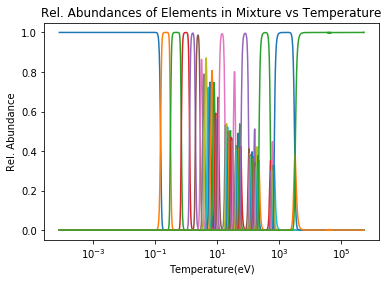
\includegraphics[scale = .75]{samarium.png}
  \centering
  \caption{Plot of relative charge state abundances vs temperature for samarium(Z = 62). There are a total of 63 charge states depicted, each color showing a new state. Relative abundance refers to abundance of each state compared to total elemental samarium abundance.}
\end{figure} 


\begin{figure}[h!]
  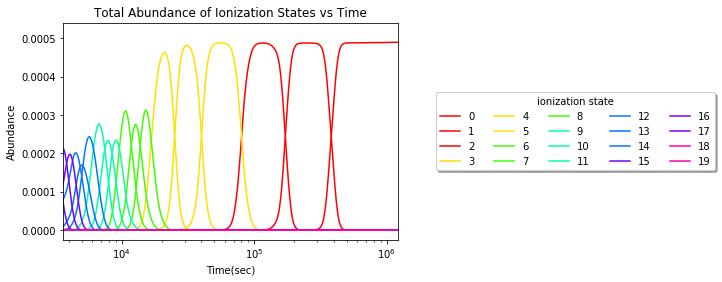
\includegraphics[scale = .65]{total.png}
  \centering
  \caption{Plot of total abundance of the lanthanides present in merger mixture vs time. Each color refers to a different state. Notice how for late times, so around 1 day, there are only 3-4 states present.}
\end{figure} 


\begin{figure}[h!]
  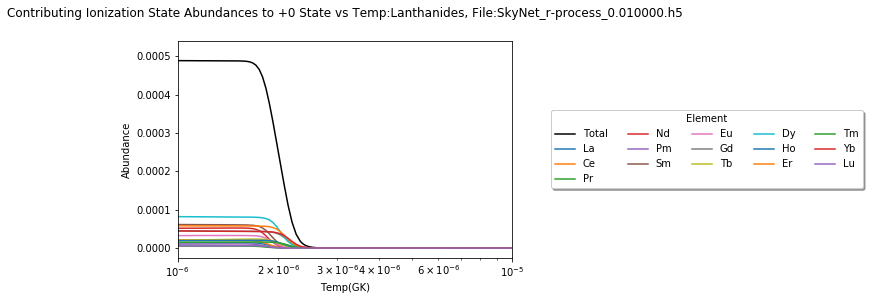
\includegraphics[scale = .6]{neutral.png}
  \caption{Plot of each lanthanide's neutral charge state abundance vs temperature. The black line is the sum of all the lanthanides' neutral abundances. }
\end{figure} 


\begin{figure}[h!]
  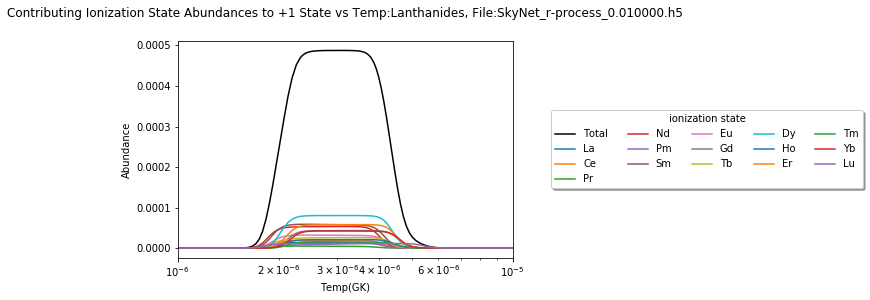
\includegraphics[scale = .6]{plus_one.png}
  \caption{Plot of each lanthanide's +1 charge state abundance vs temperature. The black line is the sum of all the lanthanides' +1 abundances. }
\end{figure} 

\pagebreak
 
\subsection{Lanthanide Electronic Configurations and Charge States}

From Skynet, it is possible to take isotopic abundances, so atoms with the same number of protons but varying neutrons, and add them together to form elemental abundances. These elemental abundances can also be constructed via the sum of all the individual charge states where the nucleus is the same but the number of electrons varies. While this is all necessary for the Saha equation calculations detailed above, one more type of abundance that is important to understand is isoelectronic abundances. Isoelectronic is when atoms have the same number of electrons orbiting the nucleus; one would expect that at really high $Z$, such as the lanthanides, that the way the electrons are arranged in their orbits might match from element to element. For example, it could be plausible that Nd-60 in the neutral charge state has the same electron configuration as Pm-61 in the +1 charge state. However, after carefully analyzing numerous electron configurations of the lanthanides based on models \url{(https://www.sciencedirect.com/science/article/abs/pii/S0092640X03000846)}, it was concluded that the most probable electron configurations for each of these elements and their charge states never matched up. In other words, it was unlikely for configuration matches such as the one listed above for Nd-60 and Pm-61 to occur.
This avenue was approached in the first place since having the same electron configuration implied rather similar spectra. Since the lanthanides are rather complex, finding such similarities amongst all the lanthanides would make studying and modeling the kilonova light curve much simpler. However, surprisingly, that was not the case. Thus, we decided to continue on our study of charge and elemental abundances.


\begin{figure}[h!]
  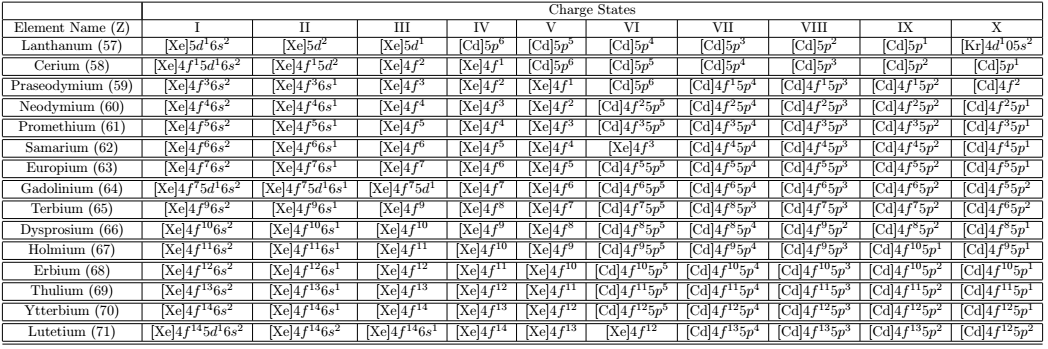
\includegraphics[scale = .65]{configurations.png}
  \caption{Table indicating the most likely electron configurations for the first ten charge states for each lanthanide. The most likely configuration was found on the NIST database.}
\end{figure}

\begin{figure}[h!]
  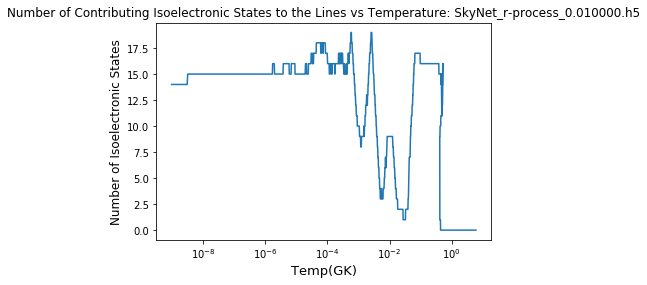
\includegraphics[scale = .6]{isoelectronic.png}
  \centering
  \caption{Plot of the number of contributing isoelectronic states present in the merger material for the lanthanides. Note that for late times/ low temperatures, there are 14 unique isoelectronic states, one for each lanthanide present. This again shows that using electron configurations is not viable. }
\end{figure}


\section{The Effect of $Y_e$ on Isotopic/Elemental Abundances}  

The electron fraction $Y_e$ is one of the input parameters for Skynet. It is one of the most important parameters considering it can only take on a range of values between 0 and 1, yet after a certain $Y_e$, the production of lanthanides drops significantly. Since the lanthanide abundances are affected by $Y_e$ values and since the lanthanide abundance alters the light curve, we can see how the light curve is affected by the starting $Y_e$ value.

\subsection{What is $Y_e$?}

The electron fraction is the density of electrons in the material relative to the density of baryons present. There are two components to this $Y_e$: the free electron fraction associated with freely moving electrons that arise from either ionization or other processes and the bound electron fraction associated with the electrons that are still in orbits about nuclei. The $Y_e$ can vary from 0 to 1 but based on numerous models and subsequent testing, it appears a $Y_e$ below .25 is indicative of a large neutron density while any $Y_e$ above that, a consequence of too much neutrino radiation, lowers the neutron density below what is needed for sufficient r-process events. \url{(https://iopscience.iop.org/article/10.3847/\\ 1538-4357/aaf054)}.


\begin{figure}[h!]
  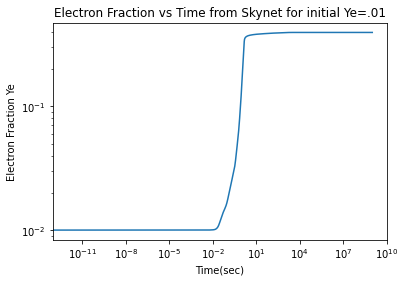
\includegraphics[scale = .75]{Ye_time.png}
  \centering
  \caption{Above is the electron fraction vs time output by Skynet for an intial $Y_e$ value of .01. The large jump in the electron fraction at approximately $10^{-2}$ seconds is from the completion of the r-process and the beginning of the lanthanides changing which charge state is dominant. }
\end{figure}


\subsection{Isotopic Abundances vs $Y_e$}

A range of $Y_e$ from .01 to .50 was used to test how the resulting isotopic and elemental abundances varied between data sets. This was done especially since the charge state abundances that are measured at late times for when the kilonova should peak(on the order of the 1st day after the merger) could be affected. This $Y_e$ range was set by Luke Roberts but also suggested by Kasen and Barnes 2013 \url{(https://arxiv.org/pdf/1303.5787.pdf)}.
After these $Y_e$ values were input into Skynet, we were able to add up all the isotopic abundances together and compare what the abundance value was at $t = 1$ day, for example, amongst various starting $Y_e$ data files. We determined the dependence of the elemental abundances on the initial $Y_e$. Knowing this is crucial to modeling kilonova since the $Y_e$ values drastically impact the abundance values, which in turn affects the spectra involved.


\begin{figure}[h!]
  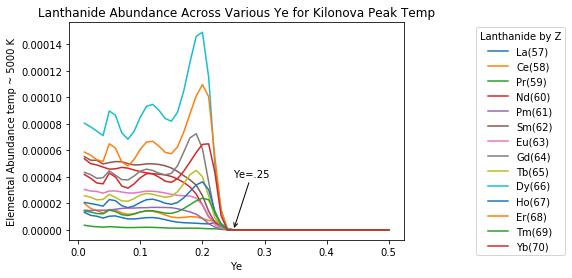
\includegraphics[scale = .6]{abun_vs_ye_temp.png}
  \centering
  \caption{Presented here are various lanthanide abundance values at the kilonova peak temperature  $\approx 5000K$ vs initial $Y_e$. The value $Y_e = .25$ is highlighted since abundances drop significantly after.}
\end{figure} 

\pagebreak 

\subsection{Defining a $Y_e$ Cutoff}

After a certain $Y_e$, the abundance starts to drop drastically, as seen by figure 18. Regardless of the element or the abundance, the lanthanide abundance values seem to drop whenever we input into Skynet an electron fraction of $Y_e$ = .25 or higher. Figure 20 also indicates this dropoff occurs for abundance values found at $t = \mathrm{1 \hspace{1 mm} day}$. This all allows one to define a $Y_e$ cutoff such that any $Y_e$ above that value would result in elemental abundances too insignificant to make a noticeable difference to the final light curve. In texts such as Kasen and Barnes 2013, this abundance threshold is $\approx 10^{-5}$.  
Look into the ipynb called “charge states abundances\_various\_Ye” for numerous graphics and implementations. Some studies are also done in the ipynb “Official \_ abundance \_ calculation \_ multiple \_ Ye \_ interpolated”. 

\section{Conclusions and Future Work}

\subsection{Main Results from Charge State Abundance Studies}

Using Skynet, a nuclear reaction network code, and the Saha equation, it is possible to model the abundances of elements and their charge states formed in neutron star mergers. For late times, the r-process has stopped, preventing any large changes in elemental abundances. As for the charge state abundances, their patterns show distinct peaks and troughs consistent with the ionization potentials of each element and each charge state, as indicated by figures 11 and 12. 
In particular, for late times, there are little to no transitions in the dominant charge state present due to the rather low temperatures. On a time scale of a day after the merger most charge states are not present besides the +3 to neutral states. 
We learned that isoelectronic states cannot be used to simplify the spectral analysis since elements with the same number of electrons have differing electronic configurations. \\

\subsection{Future work: Neodymium and Samarium Abundance Dependence on Skynet Parameters}

Fontes et al.'s recent paper \url{(https://arxiv.org/pdf/1904.13298.pdf)} discusses how, based on their kilonova models, the kilonova light curve is most sensitive to Neodymium while the rest of the lanthanides present can be modeled with just Samarium. In fact, Nd is so important that its opacity is different by one order of magnitude compared to Sm, which is supposed to be the fiducial (representative) element of the lanthanides. 

With this information in mind, it is important to see how these abundances are affected by Skynet parameters. Certain electron fractions or dynamical timescales, for example, can result in the largest Nd abundances, which means the kilonova light curve would be impacted. By compiling how the Nd and Sm abundance varies based on initial inputs, we can later figure out what the kilonova light curve will look like. 


\subsection{Future work: Studies of the $Y_e$ Cutoff vs. Skynet Parameters}

While $Y_e$ is certainly the most important Skynet parameter in altering final abundance patterns, the other parameters, notably the entropy and dynamical timescale (term used to describe how density evolves over time), must also be studied. The starting entropy and dynamical timescale can and will affect how the temperature and density values change over time, which are values necessary for charge state abundance calculations detailed in the Saha and Saha \_ mult classes. 
Thus, we plan on studying into how altering the entropy and dynamical timescale values would change the $Y_e$ cutoff needed for abundances. In the end, there will be a graphic depicting $Y_e$ as a function of these variables, and certain points or lines in a 3D graph that would correspond to critical Ye values. From this, a collection of starting Skynet parameters can be generated such that a critical $Y_e$ is always reached. By doing this, we would know which values for starting entropy and dynamical timescale have the largest impact on the $Y_e$, which ultimately indicates the impact these values can have on the abundance values. 


\subsection{Future work: Atomic Structure Codes and Beyond}

The leading groups that model kilonova light curves all use different atomic models to generate ionization potentials and atomic energy levels. With this, their associated opacities and spectra can be calculated.  These groups include Tanaka et al.\url{(https://iopscience.iop.org/article/10.3847/1538-4357/\\aaa0cb/meta)} , Fontes \url{(https://iopscience.iop.org/article/10.3847/1538-4357/ab70b9)}, and Kasen and Barnes et al. \url{(https://arxiv.org/pdf/1303.5787.pdf)}. \\

In order to generate kilonova light curves, we must track how the photons propagate through the merger material. Tracking their energy losses, trajectories, and interactions are vital to understanding which photons end up being observed outside the merger mixture using our telescopes. For the sake of convenience and error checking, we will use only the radiative transfer codes from Kasen and Barnes out of the three possible groups' codes.\\

Three unique kilonova light curves will be generated, each one differing only by the atomic structure calculations used in finding the ionization potentials and energy levels. These light curves will then be compared amongst each other and to the one from AT2017gfo. If the three curves differ by a significant amount at certain bands (wavelengths), then it is indicative that the difference in the atomic structure models are large enough to be impactful. If this is the case, we can study what atoms' structure calculations vary the most amongst these codes.\\  

An experiment would be designed to find the various energy levels and transitions of a lanthanide at various charge states. Since most charge states are not relevant at late times (around 1 day after merger), it is best to focus solely on the first 3 to 4 charge states only. An experiment could benchmark each atomic structure code with the experimental data.

\bibliography{references_technote}
\end{document}

